\subsubsection{Thermal effects and their compensation}\label{sec:tcs}
%\emph{Author(s): V.\ Fafone, A.\ Rocchi \\}

Thermal lensing due to the absorption of the laser light in the core optics of gravitational wave interferometers can represent a  limitation for 
 their operational stability and sensitivity. This effect has already been observed in the currently operating
  detectors (requiring the installation of compensation systems~\cite{ligotcs,virgotcs,Accadia2010}) and 
  will become more relevant in the second generation interferometers, due to the much higher circulating power. 
In case of ET xylophone configuration with a low-frequency cryogenic and
 a high-frequency room-temperature detector, the two interferometers show a different behaviour with respect to thermal effects. 

Due to the low power circulating in the Fabry-Perot cavities  and due to the thermal properties of silicon 
at low temperature (see table~\ref{tab:tn_T_param}), thermal effects in ET-LF will be negligible: the thermal 
gradient due to the laser power absorption results to be less than 1\,mK. On the contrary, the ET-HF 
interferometers will feature all the characteristics of an advanced detector (room temperature operation, 
high power and fused silica test masses, similar arm cavity finesse and recycling gains) and the only difference is
 the application of a LG$_{33}$ beam profile instead of TEM$_{00}$. 

In the test masses, the optical power is predominantly absorbed by the high-reflectivity 
coatings and converted into heat, producing a temperature gradient 
inside the substrate. While R\&D activities to reduce coating absorptions are ongoing (see Sec.~\ref{sec:RD}), 
values of about 0.6\,ppm have been reported in literature~\cite{pin09}. Thus, considering 3\,MW of optical 
power impinging on the test masses, the total absorbed power amounts to 1.8\,W. This is a factor of three higher than expected 
in advanced detectors~\cite{fafo08}. However, the resulting maximal temperature increase is less than 
1~degree, as shown in figure~\ref{Fig:Sec_Optics_TCS1}, compared to about 2 degrees in the advanced detectors.
 This result is mainly due to the wider intensity distribution of the LG$_{33}$.
 % in fact, in advanced detectors, where the power inside the Fabry-Perot cavities will be around 800\,kW, lower
 % by more than a factor of three than in ET-D-HF, but a TEM$_{00}$ will be used, the temperature increase is 
 %expected to be of the order of 2 degrees with the same coating absorption level~\cite{fafo08}. 
 By integration of the temperature field along the thickness of the test mass, it is possible to calculate the
  corresponding optical path length (OPL) increase. In figure~\ref{Fig:Sec_Optics_TCS2} the expected ET-HF
   optical path increase is compared to the expectation for Advanced Virgo~\cite{fafo08}: the use of LG$_{33}$ 
   modes will limit the increase of thermal effects with respect to advanced detectors to about 30\%.

\begin{figure}[!h]
\centering
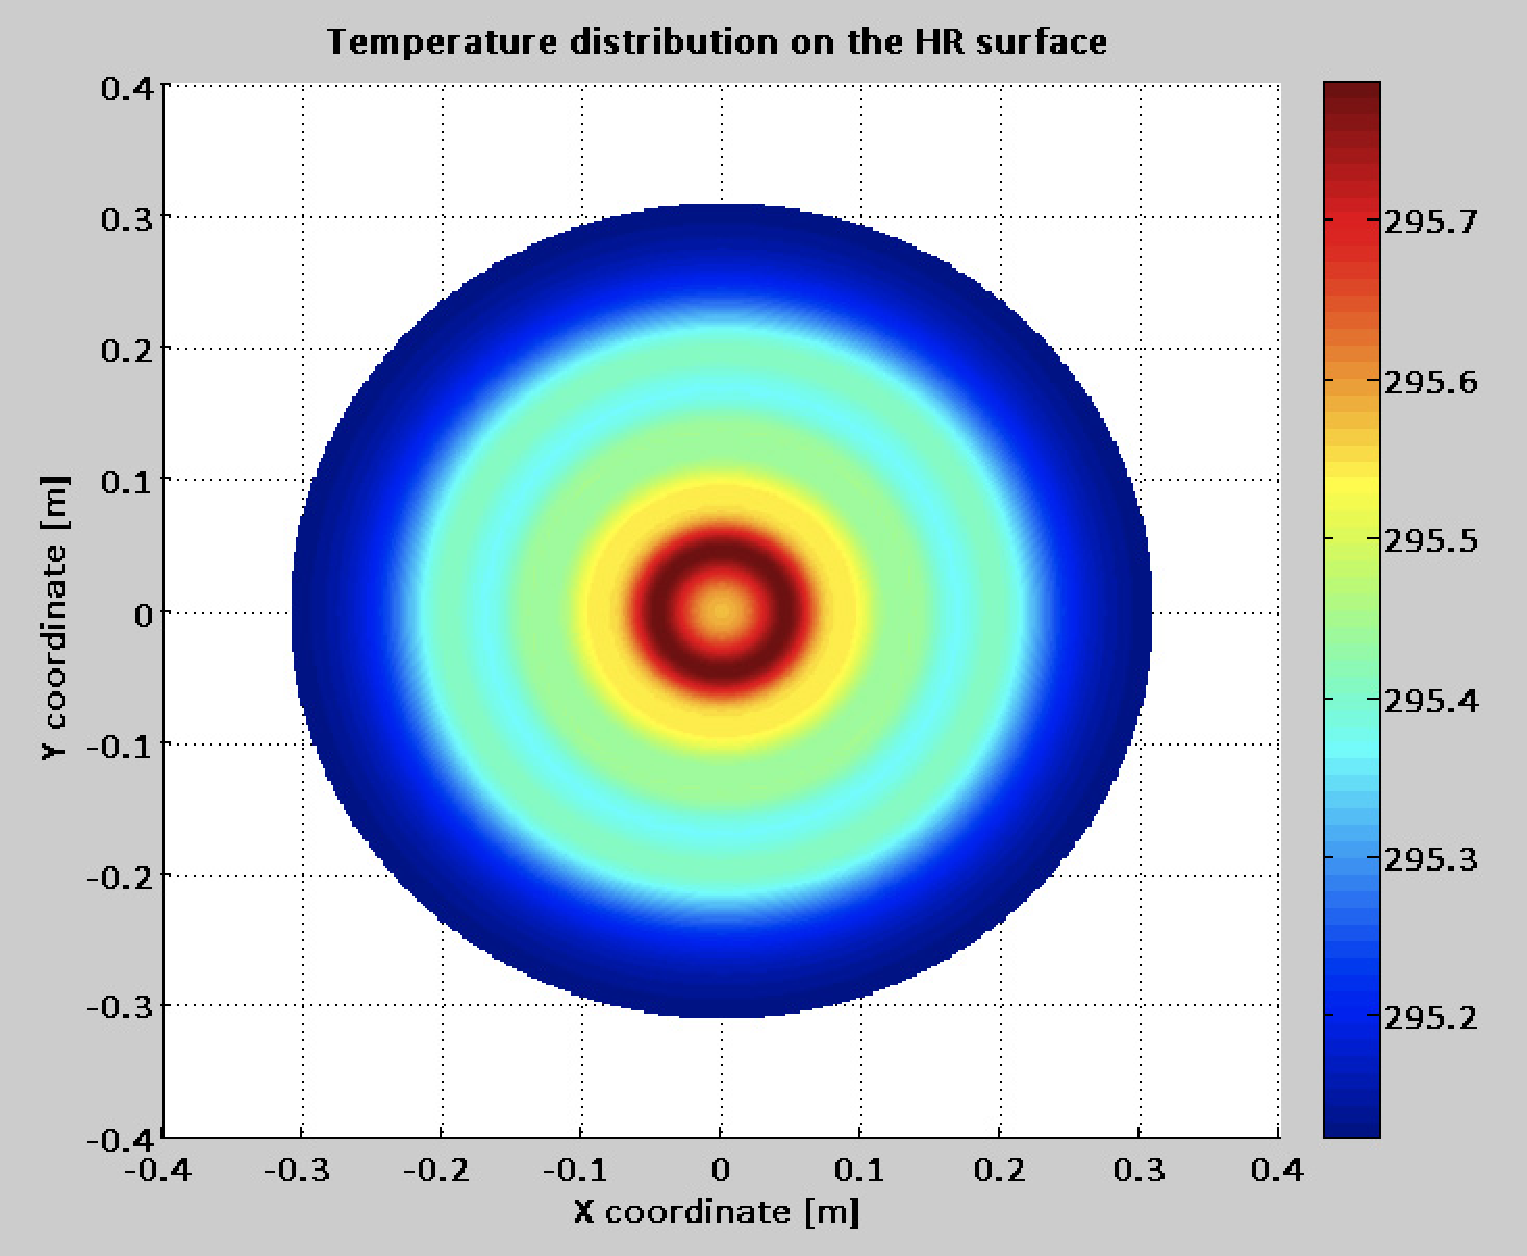
\includegraphics[width=0.4\textwidth]{Sec_Optics/TCS_1b}
\caption{Temperature distribution in ET-D-HF test mass due to the absorption of 0.6\,ppm of the arm cavity power.}
\label{Fig:Sec_Optics_TCS1}   
\end{figure}

%\textcolor{red}{Comment for the TWT: coating absorption only accounted for: FP cavity finesse and RC cavity gain needed to evaluate substrate contribution. If these parameters are not yet defined, we will add a sentence specifying the approximation used in the evaluation of thermal effects.}

\begin{figure}[!h]
\centering
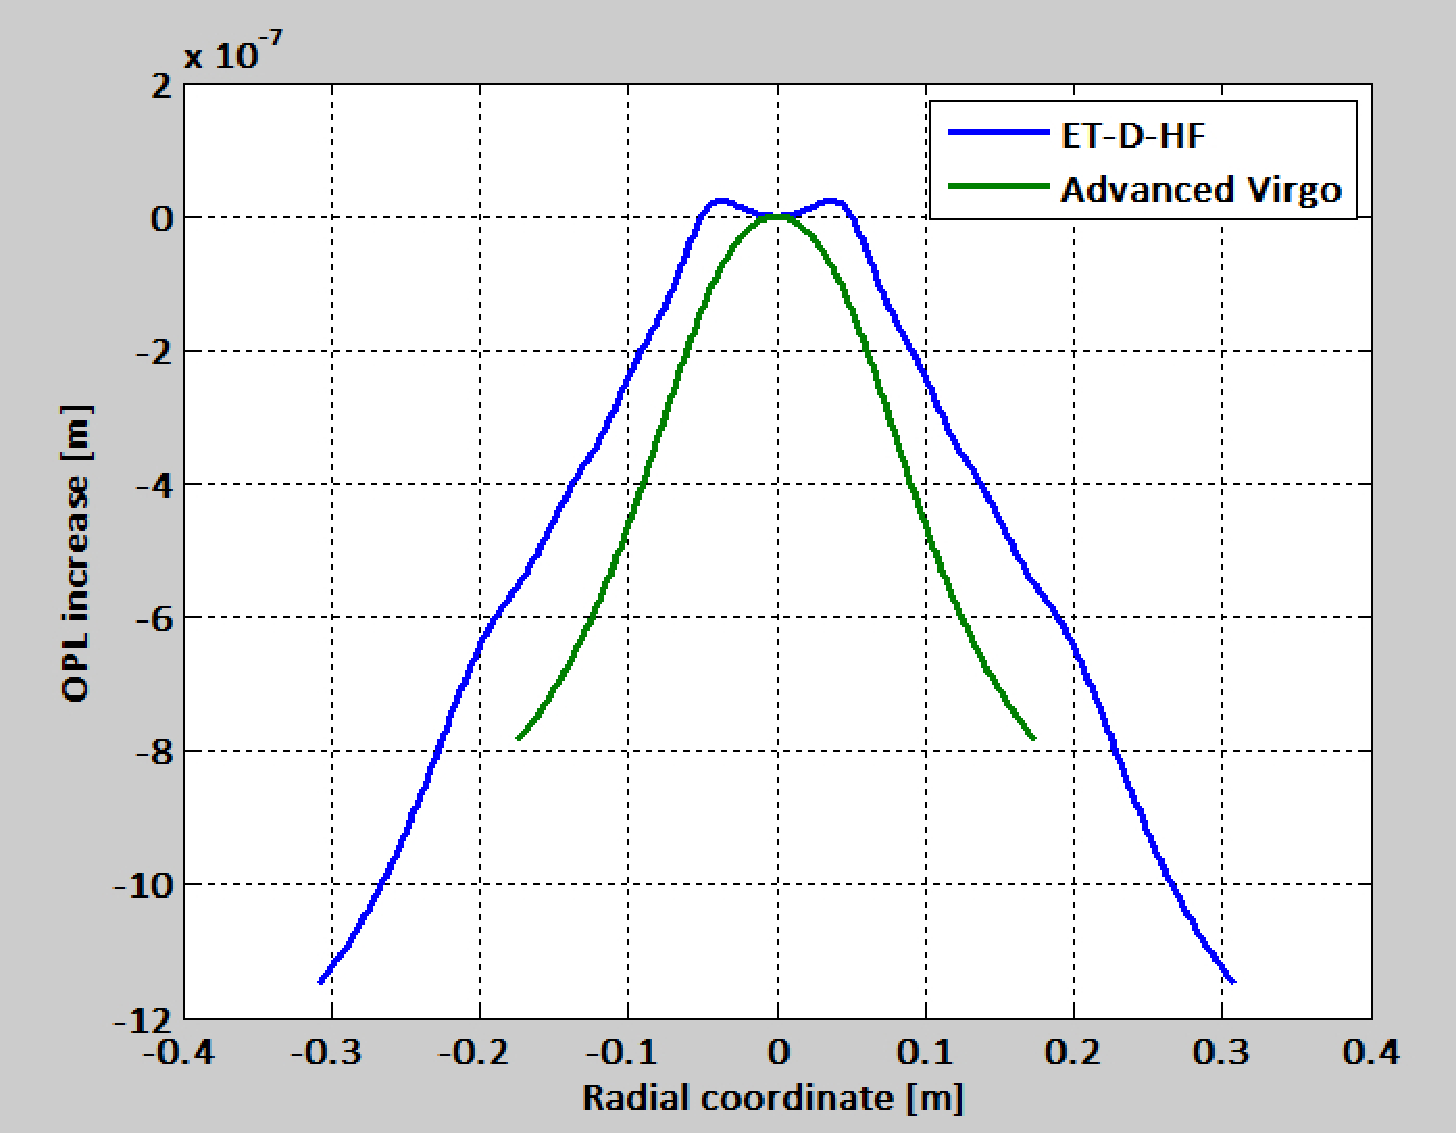
\includegraphics[width=0.45\textwidth]{Sec_Optics/TCS_2}
\caption{Optical path length (OPL) increase in ET-HF test mass (blue curve) compared to the expected values for Advanced Virgo (green curve).}
\label{Fig:Sec_Optics_TCS2}   
\end{figure}

%\subsubsection{CO$_2$ laser correction}
%\label{sec:tcs1}
%\vspace{1cm}

Since the thermal effects expected for ET-HF are  of the same order of magnitude as the ones expected for advanced detectors,
it will possible to apply for ET the same thermal compensation system (TCS) as adopted for 2$^{nd}$ generation
  interferometers. ET-HF could use a compensation plates (CP) in the recycling cavity, heated by CO$_2$ lasers,
   to cope with thermal lensing and a ring heater around each test mass to correct its thermally driven increase of radius of 
   curvature. Figure~\ref{Fig:Sec_Optics_TCS3} shows a sketch of a compensation plate  and a ring heater  around the test mass. 

\begin{figure}[!h]
\centering
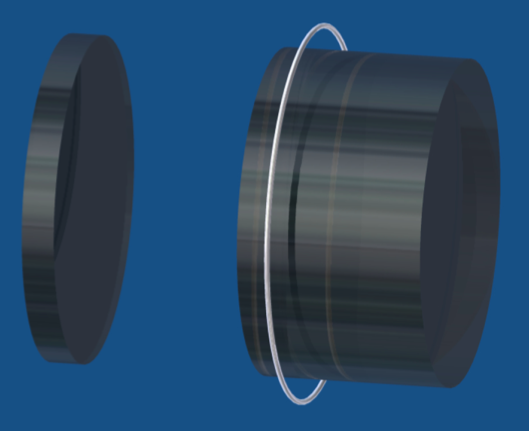
\includegraphics[width=0.35\textwidth]{Sec_Optics/TCS_3.png}
\caption{Sketch of the ET compensation plate and ring heater around the test mass (not in scale).}
\label{Fig:Sec_Optics_TCS3}   
\end{figure}

%In figure~\ref{Fig:Sec_Optics_TCS3}, the CP is thinner than the test mass. This is done to minimize the loss of compensating power from the barrel of the CP~\cite{fafo10}. On the other hand, the thickness cannot be reduced at will, since it is necessary to accumulate enough optical path lenght increase. For instance, in Advanced Virgo the CP will be 3.5\,cm thick. A reduction of the heat loss could also be achieved by gold coating the barrel of the CP (provided that the mechanical quality factor of the CP is not reduced too much).

%Since the radiative coupling between the input test mass and the compensation plate spoils the efficiency of the TCS~\cite{fafo10}, from the point of view of the thermal effects compensation, the best scheme is to suspend the CP "far" from the test mass, at a distance that minimizes the radiative coupling. 
%This would also allow to mechanically de-couple the CP from the ITM payload. 

In order to optimize the compensation level, the CP heating pattern must  account for the intensity profile of the interferometer beam. 
%will use LG$_{33}$ modes. 
A heating pattern optimization code has been developed~\cite{rocchi10}, consisting of a linear iterative optimization process based on a finite element 
analysis,
that makes use of the OPL increase ($\Delta \text{OPL}$) as error signal. At each iteration, the heating 
 pattern for the next step is calculated from the previous one and from the corresponding OPL increase:
\begin{equation}
H_{\text{path}}(n+1)=H_{\text{path}}(n)+K_L \cdot  \Delta \text{OPL}(n),
\end{equation}
where, $H_{\text{path}}$ is the CP heating pattern and $K_L$ is the loop gain. The procedure is applied 
to the complete system made of the test mass, the compensation plate and ring heater.
The result, when the compensation plate is placed sufficiently ``far'' from the ITM (thus there is no significant
radiative coupling between the test mass and the compensation plate), is shown in Fig.~\ref{Fig:Sec_Optics_TCS4}. With this 
heating pattern, TCS can flatten the optical path lenght inside the input test mass substrate up to a diameter 
of 40\,cm. This heating profile could be produced, for example, using scanning systems ( for instance making  use of  galvos
 or crossed AOMs).%, diffractive optical elements or MEMS.

\begin{figure}[!h]
\centering
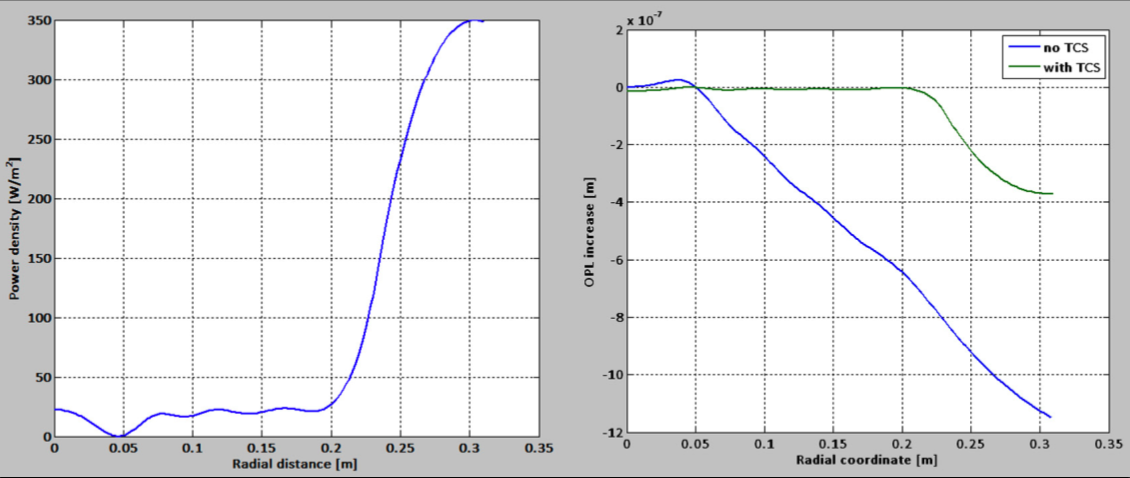
\includegraphics[width=0.7\textwidth]{Sec_Optics/TCS_4c.png}
\caption{Left picture: optimized heating pattern. Right picture: compensated optical path length (green curve) compared to the uncompensated one (blue curve).}
\label{Fig:Sec_Optics_TCS4}   
\end{figure}

Since the ET infrastructure will comprise cryogenic facilities, it could be possible to exploit them to implement a
 different technique for the compensation of thermal effects.
Such a system would aim to directly extract the heat deposited by the laser beam, before it has a chance to generate any deformation of
 the mirror. Localized heat extraction can be implemented via directional radiative cooling of the beam spot~\cite{kamp2009}. 
 For this it is required  to image a sufficiently cold black
body on the beam spot (but not on
the rest of the mirror), from a sufficiently large solid angle. Figure~\ref{Fig:Sec_Optics_TCS6} shows a conceptual design of the system.

\begin{figure}[!h]
\centering
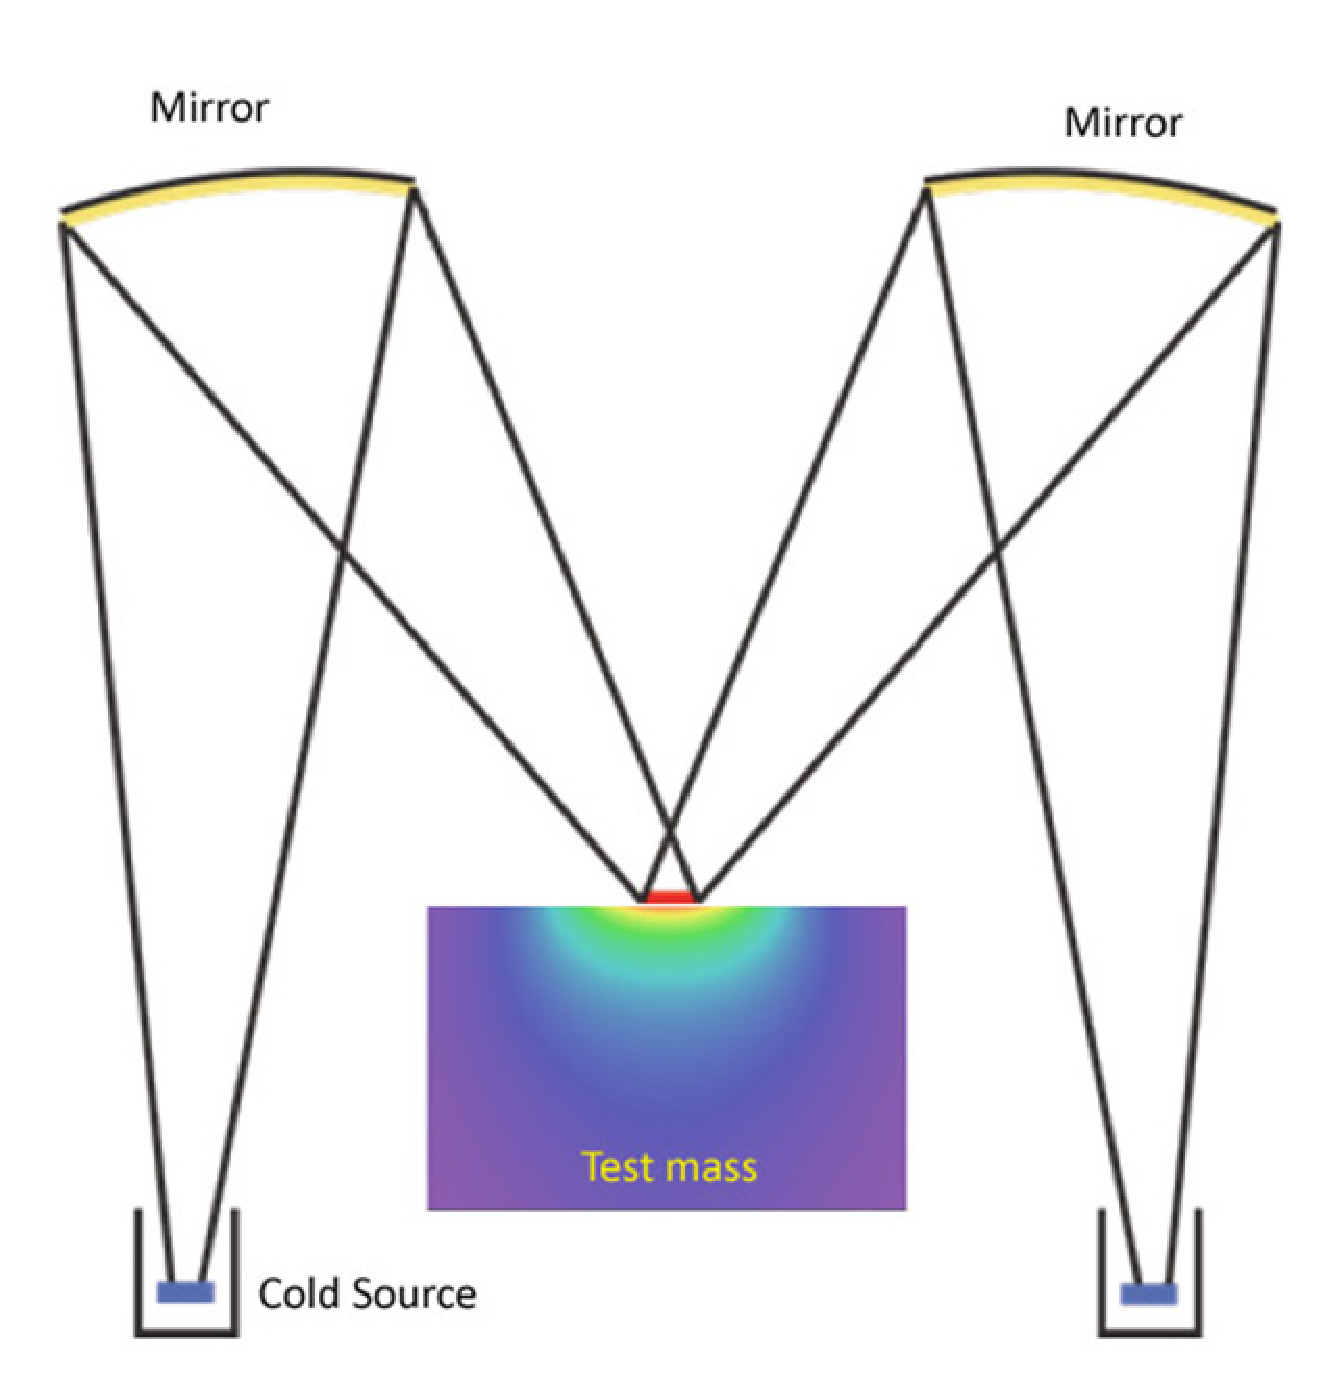
\includegraphics[width=0.3\textwidth]{Sec_Optics/TCS_6.pdf}
\caption{Conceptual scheme of the radiative cooling.}
\label{Fig:Sec_Optics_TCS6}   
\end{figure}

%The heat extraction efficiency of the technique
%drops as $T^4$, thus becoming rapidly ineffective for mirrors cooled to
%cryogenic temperatures. For this reason, this method could be used only on the high frequency component of ET, since it is a room-temperature detector.

By placing parabolic collectors behind each cold spot, the radiative coupling with the mirror 
surface is improved and it is possible to achieve  a strong reduction of the required size of the cold spot~\cite{tvpi10}. 
Such a scheme, named \emph{parobolic mirrors radiative cooling}  is shown in figure~\ref{Fig:Sec_Optics_TCS7}. 
The role of each reflector-collector couple is to build up a telescope that enlarges the radiative exchange surface 
of the cold target,
as seen by the test mass center spot. This allows for the implementation of
small cold surfaces with low cooling power and efficient temperature control.
\begin{figure}[!h]
\centering
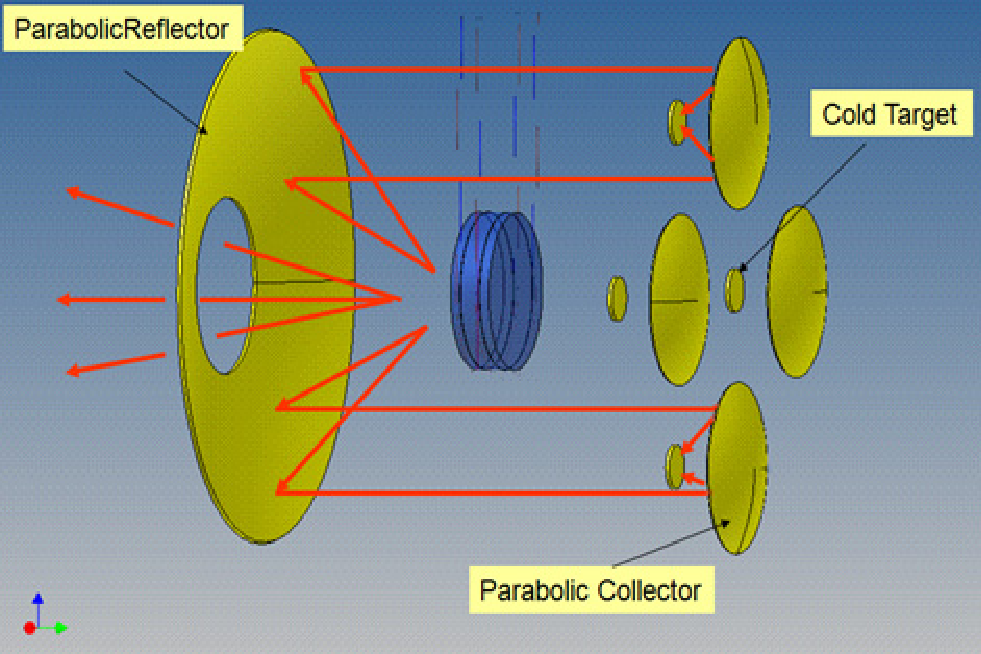
\includegraphics[width=0.4\textwidth]{Sec_Optics/TCS_7b}
\caption{Scheme of the Parabolic Mirrors Radiative Cooling.}
\label{Fig:Sec_Optics_TCS7}   
\end{figure}


The parobolic mirrors radiative cooling technique is being investigated~\cite{tvpi10} with the main aim of assessing the 
capability of the system in producing proper cooling profiles. This is done in a test facility that allows the
 imaging system and the shape of the cold spots to vary in order to modify the cooling profile and to take  the use of LG$_{33}$ modes in ET-HF
 into account.

The same concept of radiative cooling can be clearly applied to image a warm source (or an array of sources) to
 produce heating profiles onto the periphery of the test mass. This could allow us, in principle, to avoid using compensation 
 plates, provided that the noise injected by the heating system is compliant with the sensitivity requirements.

All these radiative techniques are at present under investigation. The CO$_2$ laser based 
TCS has already proven able to generate proper heating profiles.
% the radiative methods must be further studied to demonstrate their capability in producing compensating
% patterns with the accuracy required in next generations detectors. 
Again ET will be able to benefit from the vast experiences that will be gained 
by the commissioning of the TCS systems for Advanced Virgo and Advanced LIGO.

